\begin{quotation}
``\emph{学数学唯一的方式是做数学。}''

{\ttfamily ``The only way to learn mathematics is to do \\mathematics.''\\
--- Paul Halmos}

``\emph{数学就像尼罗河一样,从微不可察到浩瀚博大。}''

{\ttfamily ``The study of mathematics, like the Nile, begins \\
in minuteness but ends in magnificence.''\\
--- Charles Caleb Colton}
\end{quotation}

\section{课程:数学思想方法 -- 1 函数与方程}
\subsection{转化为方程}
网课中提到了这样一个有趣的题目:已知
\[
\frac{\sqrt{5}b - c}{5a} = 1
\],
$a,\ b,\ c \in \mathbb{R}$, 则\(b^2\)与\(4ac\)的大小关系为?

要考虑\(b^2\)与\(4ac\)的大小关系,可考察\(b^2 - 4ac\)的正负。这不是别的,正是一元二次方程的
判别式的形式。故考虑把题目中的等式转化为一元二次方程的形式。我们有:
\begin{align}
(a &\neq 0) \nonumber \\
\sqrt{5}b - c &= 5a \nonumber \\
\sqrt{5}^2a - \sqrt{5}b + c &= 0
\end{align}
即一元二次方程\(ax^2 + bx + c = 0\)在$\mathbb{R}$上至少有一个解$-\sqrt{5}$。
且由于我们的每一步转化都有必要且充分的关系,
故\(b^2 \geq 4ac\)

\subsection{更换自变量}
在一些带有参变量的一元二次不等式里,可以更换自变量,把一元二次不等式转化为线性函数来求解。
比如网课中提到的已知\(7x - 2 > (x^2 - 1)m\)对\(m \in [-2,2]\)恒成立,求实数$x$的取值范围。
把$m$作为自变量,就可以得到关于$m$的线性函数。具体做法不是我们讨论的重点,今转而证明其必要充分性。
\begin{proof}
首先题目的意思是对\(\forall m \in [-2,2]\),求$x$的集合,使其中的$x$都满足
\(7x - 2 > (x^2 - 1)m\). 我们通过更换自变量的做法得出的结果是一个$x$的集合,其中的$x$都满足
了对\(\forall m \in [-2,2]\),\(0 > (x^2 - 1)m - 7x + 2\)。由于
\(7x - 2 > (x^2 - 1)m\)与\(0 > (x^2 - 1)m - 7x + 2\)互为必要且充分的条件,故这种方法做
出来的就是解。
\end{proof}

\subsection{数列最值}
对于一个数列,考察其最值的方法也可以参照考察函数最值的方法,因为数列也可以被看成定义在整数集的某
个子集上的函数,和一般的函数来说区别只是定义域不连续。比如网课中的某道题的一部分:求
\[
\sigma_n = \sum_{i = n+1}^{2n}{\frac{1}{i}}
\]的下确界.\footnote{界的概念虽然未涉及,但比较基础,我们就直接用了。这里简单介绍下,如果某个数集
$\mathbb{S}$中的所有元素$\leq\ (\geq)$某个数$m(n)$则$m(n)$是$\mathbb{S}$的上界(下界)。
上界(下界)中如果存在最小(最大)的数$M(N)$则数$M(N)$是$\mathbb{S}$的上(下)确界。}

讨论函数最值时有时我们使用单调性判断,而单调性可通过取$x_1,x_2$做差判断,我们把这个方法运用到这
题上。令\(d = \sigma_{n+1} - \sigma_n\),考察$d$的正负。我们有
\begin{align}
d 
&= \frac{1}{2n+1} + \frac{1}{2n + 2} - \frac{1}{n + 1} \nonumber \\
&> \frac{1}{2(n + 1)} + \frac{1}{2(n + 1)} - \frac{1}{n + 1} = 0
\end{align}
就明白$\sigma_n$递增,于是其下确界是$\sigma_1 = \frac{1}{2}$.

\section{课程:数学思想方法 -- 2 函数与方程在几何中的应用}
课程中提到了这样一道题:
已知正方体的棱长为$a$,平面$\alpha$与每条棱所在直线成角都相等,$\cdots$。
课程里直接给出了一个特例平面,并说把这个平面平移,而没有讲$\alpha$是怎么被求出来的。现在我们来做一
下。

首先,让正方体一个顶点上的三条棱都放在坐标轴上,这样,显然,每条棱所在直线都和坐标轴的其中一条平行。
这样只要找到$\alpha$与三条坐标轴成的角相等就好了。这即是让它的法向量$\vec{n_{\alpha}}$与
\((0,0,1),\ (0,1,0),\ (1,0,0)\)成的角都相等。设
\[
\vec{n_{\alpha}} = (x,y,z)
\]
则$x=y=z$,便取$\vec{n_{\alpha}} = (1,1,1)$就好了。

\section{课程:数学思想方法 -- 3 构造}
\subsection{构造向量解题}
可能会遇到这种题目,给出了如下条件:
\begin{equation*}
\begin{cases}
\sin{\alpha_0} + \cdots + \sin{\alpha_n} = a \\
\cos{\alpha_0} + \cdots + \cos{\alpha_n} = b
\end{cases}
\end{equation*}
这时可构造向量\(\vec{v}_0 = (\sin{\alpha_0}, \cos{\alpha_0}), \cdots, 
\vec{v}_n = (\sin{\alpha_n}, \cos{\alpha_n})\)并做和
\(\vec{n} = \vec{v}_0 + \cdots + \vec{v}_n\)来研究。此时\(\vec{n}=(a,b)\)。

例:若
\begin{equation}
\begin{cases}
\sin{\alpha} + \sin{\beta} + \sin{\gamma} = 0 \\
\cos{\alpha} + \cos{\beta} + \cos{\gamma} = 0
\end{cases}
\label{eq:exam1}
\end{equation}
且\(0 < \alpha < \beta < \gamma < 2\pi\),求\(\beta - \alpha\)。

\textbf{解}:
令\(\vec{\varphi}_\alpha = (\sin{\alpha}, \cos{\alpha}), \cdots, 
\vec{\varphi}_\gamma = (\sin{\gamma}, \cos{\gamma})\), 
\(\vec{s} = \vec{\varphi}_\alpha + \vec{\varphi}_\beta + \vec{\varphi}_\gamma\)
则由\ref{eq:exam1}得,\(\vec{s} = \vec{0}\),或表示为
\(\vec{\varphi}_\gamma = - (\vec{\varphi}_\alpha + \vec{\varphi}_\beta)\)。
现在由这个关系推导角的关系。首先考虑一个特殊情况,当\(\gamma = \frac{3}{2}\pi\)时,如图
\ref{fig:exam1},参见各个向量的情况。

\begin{figure}[!hbtp]
\begin{center}
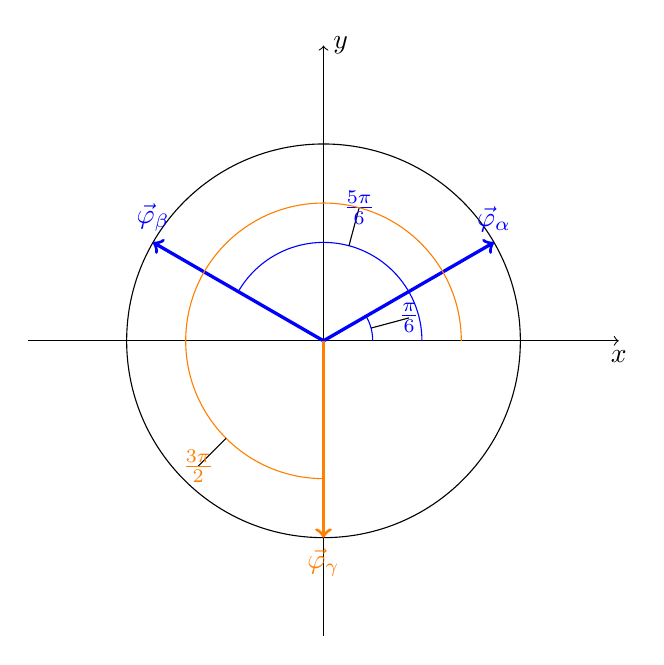
\begin{tikzpicture}[scale=2.5]
\draw[->] (-1.5,0) -- (1.5,0) node [anchor=north] {$x$};
\draw[->] (0,-1.5) -- (0,1.5) node [anchor=west] {$y$};

\draw (0,0) circle [radius=1];

\draw[color=blue, very thick, ->] (0,0) -- (30:1)
 node [anchor=south] {$\vec{\varphi}_\alpha$};
\draw[color=blue, very thick, ->] (0,0) -- (150:1)
 node [anchor=south] {$\vec{\varphi}_\beta$};
\draw[color=orange, very thick, ->] (0,0) -- (270:1) 
node [anchor=north] {$\vec{\varphi}_\gamma$};

\draw[color=blue] (2.5mm,0) arc 
[start angle=0, end angle=30, radius=2.5mm, thick];
\draw (15:2.5mm) -- +(15:2mm) node [color=blue] {$\frac{\pi}{6}$};
\draw[color=blue] (5mm,0) arc 
[start angle=0, end angle=150, radius=5mm, thick];
\draw (75:5mm) -- +(75:2mm) node [color=blue] {$\frac{5\pi}{6}$};
\draw[color=orange] (7mm,0) arc 
[start angle=0, end angle=270, radius=7mm, thick];
\draw (225:7mm) -- +(225:2mm) node [color=orange] {$\frac{3\pi}{2}$};

\end{tikzpicture}
\end{center}
\caption{
\(\vec{\varphi}_{\alpha,\beta,\gamma}\)的关系当\(\gamma = \frac{3}{2}\pi\)时}
\label{fig:exam1}
\end{figure}

这时很易看出\(\beta - \alpha = \frac{\pi}{3}\)。随后改变$\vec{\varphi}_\gamma$,
另外两向量的位置唯一确定,且相对位置不变,相当于原图旋转了一些。故无论如何
\(\beta - \alpha = \frac{\pi}{3}\)。

\subsection{构造对偶式}
我们在网课里看到了一个有趣的解法,背后的原理暂时没有弄明白,先把做法记下。

例:
试求\(\sin^2{20\mdeg} + \cos^2{50\mdeg} + 
\sin{20\mdeg}\cos{50\mdeg}\)。

\textbf{解}:

令\(\alpha = \sin^2{20\mdeg} + \cos^2{50\mdeg} + 
\sin{20\mdeg}\cos{50\mdeg}\), 把\(\alpha\)中的sin换成cos,cos换成sin,就
得到了所谓的对偶式\(\beta = \cos^2{20\mdeg} + \sin^2{50\mdeg} + 
\cos{20\mdeg}\sin{50\mdeg}\).

我们有
\begin{align}
\alpha + \beta
&= (\sin^2{20\mdeg} + \cos^2{20\mdeg}) + (\sin^2{50\mdeg} + 
\cos^2{50\mdeg}) \nonumber \\
&+ (\sin{20\mdeg}\cos{50\mdeg} + 
\cos{20\mdeg}\sin{50\mdeg}) \nonumber \\
&= 2 + \sin{70\mdeg}
\end{align}
\begin{align}
\alpha - \beta
&= (\sin^2{20\mdeg} - \cos^2{20\mdeg}) + (\sin^2{50\mdeg} - 
\cos^2{50\mdeg}) \nonumber \\
&+ (\sin{20\mdeg}\cos{50\mdeg} - 
\cos{20\mdeg}\sin{50\mdeg}) \nonumber \\
&= -\cos{40\mdeg} + \cos{100\mdeg} - 
\sin{30\mdeg}
\end{align}
注意到
\begin{align*}
\cos{40\mdeg} = \cos{(70\mdeg - 30\mdeg)}\\
\cos{100\mdeg} = \cos{(70\mdeg + 30\mdeg)}
\end{align*}
故
\begin{equation}
\alpha - \beta = -2\sin{70\mdeg}\sin{30\mdeg} - \frac{1}{2}
\end{equation}
则
\begin{align}
\alpha
&= \frac{1}{2}(\alpha + \beta + \alpha - \beta) \nonumber \\
&= \frac{3}{4}
\end{align}

我们很好奇这是不是一个特殊的例子才成立。于是我们把\(30\mdeg,\ 50\mdeg\)换成一般角\(A,\ B\),
并令
\begin{align*}
m &= \sin^2{\alpha} + \cos^2{\beta} + \sin{\alpha}\cos{\beta} \\
n &= \cos^2{\alpha} + \sin^2{\beta} + \cos{\alpha}\sin{\beta}
\end{align*}

则,很易通过之前的推导看出,
\begin{align*}
m + n &= 2 + \sin{(\alpha + \beta)} \\
m - n &= 2\sin{(\alpha - \beta)}\sin{(\alpha + \beta)} + \sin{(\alpha - \beta)}
\end{align*}

这样,只有\(2\sin{(\alpha - \beta)} = -1\)是,m才能被求出,或者当\\
\(\sin{(\alpha - \beta)},\ \sin{(\alpha + \beta)}\)都可被求出时也行。

\subsection{构造几何图形}
课程里提到了一个比较经典的题:给出一个三角形的一角和其对边,求它的面积的最大值。课程中给了构造其
外接圆的方法。首先由正弦定理,确定其一角和对边的话,其外接圆的半径便是常数了。图
\ref{fig:ConstructGeometry}展示了当定角为$\frac{\pi}{3}$,对边为2时的情况。显然,
\(S_{\triangle ABC}\)最大仅当C在最上面。

\begin{figure}[!hbtp]
\begin{center}
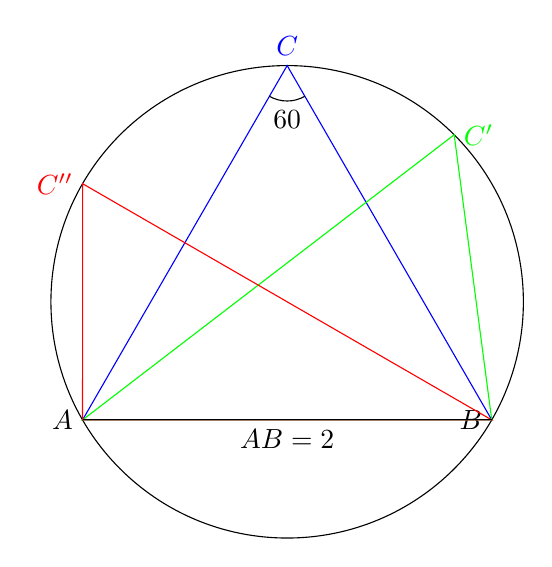
\begin{tikzpicture}[scale=1.5]
\coordinate [label=left:{$A$}] (A) at (210:2);
\coordinate [label=left:{$B$}] (B) at (-30:2);

\draw (0,0) circle [radius=2];
\draw[color=blue] (A) -- (B) -- (90:2) node[anchor=south] {$C$} -- cycle;
\draw[color=green] (A) -- (B) -- (45:2) node[anchor=west] {$C'$} -- cycle;
\draw[color=red] (A) -- (B) -- (150:2) node[anchor=east] {$C''$} -- cycle;
% make AB black.
\draw (A) -- (B);

\node[anchor=north] at (0,-1) {$AB=2$};

\draw (90:2) +(240:3mm) arc [start angle=240, end angle=300, radius=3mm];
\node[anchor=north] at (0,1.7) {$60\mdeg$};

\end{tikzpicture}
\end{center}
\caption{构造外接圆}
\label{fig:ConstructGeometry}
\end{figure}

不过构造要注意的一点,课程里没有提,就是,构造的东西是否和它唯一对应。首先,圆上这样的每一个三角形
都满足题目条件,只因弦对的圆周角相等。另一方面,任意的这样三角形都可被这样放在圆上,这比较显然。故
构造出来的东西与题目唯一对应。

这做法比较简单易懂,然而我们想转而考察纯代数求其最大值。
首先,无论如何,\(S_{\triangle ABC} = \frac{ab\sin{C}}{2}\),而\(\sin{C}\)是常数,
故只要考察$ab$即可。
依正弦定理,
\begin{equation}
\frac{2}{\frac{\sqrt{3}}{2}} = \frac{b}{\sin{B}} = \frac{a}{\sin{A}}
\end{equation}
则
\begin{align*}
\frac{ab}{\sin{A}\sin{B}} &= \frac{16}{3} \\
ab &= \frac{16}{3}\sin{A}\sin{B}
\end{align*}
又
\[
A = \frac{2\pi}{3} - B
\]
则
\begin{equation}
ab = \frac{16}{3}\sin{(\frac{2\pi}{3} - B)}\sin{B}
\end{equation}
剩下求最大值就很好求了,只需注意下$B$的范围即可。

让我们看一下另一个例题。试求
\[
f(x) = \frac{1-\sqrt{2}\sin{x}}{4-\sqrt{2}\cos{x}}
\]
的最值。
我们发现\(\sin{x}\)和\(\cos{x}\)前面的系数相等,这意味着对任意的$x$,它们组合起来可表示
在一个圆的某个点,而反过来,圆上的任意一点与 \\
\((\sqrt{2}\cos{x}, \sqrt{2}\sin{x})\)对应。于是考虑构造圆\(x^2 + y^2 = 2\)。而
\(f(x)\)不是别的,正是圆上一点P与点(4, 1)所确定直线的斜率。故可从几何关系上考虑此问题。图
\ref{flg:ConstructStraightLine}展示
了构造出的图形。
\begin{figure}[!hbtp]
\begin{center}
\begin{tikzpicture}
\coordinate [label=right:{$A(4,1)$}] (A) at (4,1);

\clip (-2,-2) rectangle (5.2,2.2);
\draw[->] (0,-2) -- (0,2) node[anchor=west] {$y$};
\draw[->] (-2,0) -- (5,0) node[anchor=north] {$x$};

% we must use node here for tangent coordinate system to work.
\node[circle, draw] (O) at (0,0) [inner sep=0, minimum size=2.82843cm] {};

\draw[color=red] (A) -- (tangent cs:node=O, point={(A)}, solution=1);
\draw[color=red] (A) -- (tangent cs:node=O, point={(A)}, solution=2);

\node[anchor=west] at (-60:1.414cm) {$O: x^2 + y^2 = 2$};

\end{tikzpicture}
\end{center}
\caption{构造圆与直线转化为斜率问题}
\label{flg:ConstructStraightLine}
\end{figure}

很易求出切线的斜率
\[
k = \frac{4 \pm \sqrt{30}}{14}
\]
故\(f(x)\)的最值分别为\(\frac{4 - \sqrt{30}}{14},\ \frac{4 + \sqrt{30}}{14}\).

\subsection{构造二项式}
一些关于求组合数的题目也挺有趣的,有些是构造二项式求解。比如:求
\[
\sum_{i=0}^n{\text{C}_{n}^i}
\]
便可通过构造\((1+x)^n\)并令\(x=1\)来求解。

然而课程中没有给上式,可能是觉得它太简单,转而给了一个这样的式子:
\[
\sigma = \sum_{i=0}^9{\text{C}_{10}^i\text{C}_{10}^{i+1}}
\]
在构造之前,先使用了组合数的性质把$\sigma$改写为
\[
\sigma = \sum_{i=0}^9{\text{C}_{10}^i\text{C}_{10}^{9-i}}
\]
这使得每一个乘积的上标之和都是9。随后构造\((x+1)^{10}(x+1)^{10}\),依二项式定理展开,得
\[
(\sum_{i=0}^{10}{\text{C}_{10}^ix^i})(\sum_{i=0}^{10}{\text{C}_{10}^ix^i})
\]
这让我们很易看出,在上标之和等于9得时候,$x$的次数也是9。而\(\sigma\)不是别的,正是\(x^9\)的系
数。现在把\((x+1)^{10}(x+1)^{10}\)合并为\((x+1)^{20}\),并求其中\(x^9\)的系数就是
\(\sigma\)了。显然,这系数是\(\text{C}_{20}^9\).

\section{课程:数学思想方法 -- 4 转化}
吐槽下,网课里说是转化与化归,竟然好多是转化成特殊值\footnote{这里的特殊值的意思是,不严谨的特殊
值,比如符合这个条件的情况中只取了一种,用这一种情况解答。}做的,我们不喜欢这样,我们觉得这样不是在做数
学,只是为了得分。既然你这样做,那我们就用超纲知识解了,请看网课里这道题:

设函数\(f(x) = \ln{x} + \frac{m}{x},\ m \in \mathbb{R}\),若
\[
\forall b > a > 0,\ \frac{f(b) - f(a)}{b - a} < 1
\]
恒成立,则$m$的取值范围是?

\textbf{解}:
显然$f(x)$在$[a,b]$上连续,$(a,b)$上可微,
依拉格朗日中值定理,
\begin{equation}
\frac{f(b) - f(a)}{b - a} = f'(c),\ c \in (a,b)
\end{equation}
另外,由于$f'(x)$也是连续的($x>0$),这使得对任意定义域上的$t$,可找到这样的
$b > a > 0,\ t \in (a, b)$,使得
$f'(t)$与$\frac{f(b) - f(a)}{b - a}$任意接近。
上面的讨论是在说明
\begin{itemize}
\item 对$\forall b > a > 0$,都可找到$c>0$,使$\frac{f(b) - f(a)}{b - a}$与$f'(c)$任意
接近(我们得到的是更严格的相等)。
\item 对$\forall c>0$,都能找到$b > a > 0$,使$\frac{f(b) - f(a)}{b - a}$与$f'(c)$任意
接近。
\end{itemize}
于是很易看出$f'(x)$的确界(如果有)与$\frac{f(b) - f(a)}{b - a}$的确界(如果有)相等。
而
\begin{equation}
f'(x) = \frac{1}{x} - \frac{m}{x^2}
\end{equation}
有上确界$\frac{1}{4m}$当$m > 0$时,于是$\frac{f(b) - f(a)}{b - a}$的上确界也是这个。
现在考察它能不能达到这个。事实上,这是不可能的,因为对某个
$\frac{f(b) - f(a)}{b - a} = f'(c)$,总能找到
\begin{equation}
f'(c') > f'(c),\ \frac{f(b') - f(a')}{b' - a'} = f'(c')
\end{equation}
于是接下来只要让$\frac{1}{4m} \leq 1,\ m > 0$就好了。

\subsection{转化为裂项相消}
这里说一下一个不是网课内容里的东西。
对形如$(an + b)c^n$的数列的求和,我们往往使用错位相减法。然而,在还未放假的时候,我们的数学老师转
而介绍了这样一种方法:用裂项相消求和。首先我们想一下裂项相消的条件。
首先要求$\sum_{i=1}^{n}{a_n}$的话,裂项一般是把$a_n$裂成$b_{n+1} - b_n$的形式。
这样$a_n + a_{n+1}$就能消去$b_{n+1}$。
于是问题就成为了求$b_n$使$(an + b)c^n = b_{n+1} - b_n$。首先考虑的是,$b_n$是不是也可以被
写成$(an + b)c^n$的形式。原理上来看,这是可以的。如果令$b_n = (a'n + b')c'^n$,那么
\[
b_{n+1} - b_n = c'^n[a'(c'-1)n + c'a' + c'b' -b']
\]
令
\begin{equation}
\begin{cases}
c' = c\\
a'(c'-1) = a\\
c'a' + c'b' - b' = b
\end{cases}
\end{equation}
就得出了一个符合条件的$b_n$。可能还有其他符合条件的,不过我们这里不需要求出其它的,只要保证充分性
就足够了。

这样,
\begin{equation}
\sum_{i=1}^{n}{a_n} = b_{n+1} - {b_1}
\end{equation}

\section{课程:数学思想方法 -- 5 分类讨论}

\subsection{排列组合中的分类讨论}
课程里大部分的分类讨论没什么好说的...分类几乎是只要基础扎实就很易看出的。我们一般在分类讨论上遇到问
题最多的地方就是在排列组合题上。经过一段时间的思考,我们总结出了一种方法能比较稳定地确定做排列组合题
的正确性。

大多数排列组合题的要求都是从一个给定集合中按某种题目要求的\emph{选法},取出一些元素,按照一定的顺
序,把它们排列起来。如果把这样一种排列叫做一种\emph{情况},题目一般是让我们求所有情况的个数。然而
经常出现根据题目要求的选法很难直接求出个数,于是我们常常构建一个和题目\emph{等价}的选法,用这个选
法求情况的个数。然而我们发现,光要求这个选法和题目的选法等价还是不够的,这可能会导致求出的情况个数变
多。我们对于两个选法等价的定义是:
\begin{itemize}
\item 给定的选法1得出的每一种情况都可以通过选法2得出,且
\item 选法2得出的每一种情况都可以通过选法1得出
\end{itemize}
为什么在实际中会导致求出的情况个数变多呢?以及,最奇怪的问题是,为什么当求出的情况个数不同时,
为何只会变多不会变少呢?毕竟这个选法等价关系和顺序无关啊\footnote{选法A等价于选法B与选法B等价
于选法A没区别}。为了回答这两个问题,我们思考了挺长的一段时间才发现了如下问题:首先题目的选法很特殊,
一般是给出了情况的限制条件 --- 既是,定义了什么样的情况满足题目要求。然而我们想出的选法却一般有这
样的特点:先分类\footnote{这也是为什么我们把这一部分放到分类讨论里面的原因。},再在每个分出的类别下
按某种选法选出满足题目要求的情况。这导致了可能出现在不同的分类下的选法选出了一样的情况,然而这并不
和选法等价冲突;而另一方面,题目给出的定义式选法不可能导致这种后果(或者说,定义本身就使得确定情况的
唯一性是我们的责任而不是题目的)于是这导致了我们的问题。

意识到这两个问题和它们的诱因后,我们又在想出的选法后加了一个条件,不仅要和题目选法等价,还要保证选出
的情况是唯一的,即不可能在两种不同的情况下,使用该选法选出同样的情况。或者即使该选法出现了重复的情
况,也可以很易通过一些方式在情况的数目中去掉它们。

让我们来看一些例子:

网课中的一道题是这样的:
有8张卡片分别标有数字$1,2,\cdots,8$,今从中取出6张排成3行2列,且只有第二行的两张卡片数字之和为
5,则不同的排法有?种?

很易看出这题目给了我们满足条件的情况的定义,让我们求情况数。现在我们来找一种选法。找到的选法为:
\begin{enumerate}
\item 先根据第二行的两张卡片数字之和为5,得出第二行要么是1,4要么是2,3,这情况有
$2! \times 2 = 4$种,
\item 之后我们有6张卡片要被填进4个空里,然而这里绝不是选4个填进去这么简单,因为题目中的``只有''
暗示了我们如果如果第二行是1,4,2,3就不能在另一行出现,反过来也一样。于是我们这里再分一次类,不妨以
第二行是2,3为例。则分1,4都被用到;1,4中只有一个被用到;1,4 \\
都没有被用到这3种情况。
\item 当1,4都被用到时,它们不能在一行。可以从所有求得的结果中删去它们在一行的结果,这做法比较好
理解。于是先从剩的4个数5,6,7,8中选2个出来有\(\text{C}_4^2=6\)种结果,之后得到了要用的4个数做
全排列 \\ 
\(4!=24\),再删去1,4在一行的情况\(2! \times 2! \times 2 = 8\),其中一个\(2!\)是1,4
的行排列,另一个是另外两个数的行的排列,最后的2是行上下颠倒。即选出的4个数的情况只有
\(24 - 8 = 16\)种。一乘得到\(16 \times 6 = 96\)种,
\item 当1,4中只有一个被用到时,从剩的4个数中选3个有\(\text{C}_4^3=4\)种,再对4\\
个数做全排列,然后一乘得\(24 \times 4 = 96\)种,再$\times 2$(因为1,4各一次)得结果192,
\item 当1,4一个都没有被用到时,直接做全排列\(4!=24\)就是最后的结果。
\end{enumerate}

现在我们考察这选法是否满足我们的要求。
首先证明它和题目的选法等价。首先题目得出的每一种情况都能被这选法得出,因为我们第一分类包含了所有的
情况,第二分类里面的情况都被排列/组合完全包含了。然后我们这选法得出的每一种情况显然都符合题目。

下面来看它是否能使选出的情况唯一。这是比较明显的。因为首先我们分的情况是互斥的,比如当1,4都被用到
时就不可能是1,4中只有一个被用到。然后在各个情况之中,排列/组合保证了得出情况的唯一性。

于是根据这选法来求情况数,是\(4 \times (24+192+96) = 1248\)种。

在这个考察过程中,发现了两点,第一:排列组合使各个分类下的细节计算得出情况的唯一性被保证,我们这里详
细提及,以后用到只要心里记得就好了。第二:如果分类是互斥的,分类的情况的唯一性就变得显然了,但这可能
并不会使问题更简单,因为有时我们改变分类使分类唯一时分类里面会变得复杂,这样本质上我们并没有消灭问
题而是把它推到了下一层,应该根据具体情况来定怎么分类。

\section{课程:数学思想方法 -- 6 放缩}
一些放缩用到的知识都比较基础,比如在分式中放大/缩小分母,在和式中放大/缩小每一项。这些的原理没什么
好说的,不过在应用中往往需要大量的尝试和经验来明白放缩到什么地步,这就很难能被总结出来。

在这一节,我们转而记载一些不是网课上,而是一些很经典的运用放缩法的证明,希望我们能从这些例子中总结出
一些有用的东西。

\subsection{伯努利不等式}
我们来看一下一个数学中很有名的被以\emph{Jacob Bernoulli}之名命名的伯努利不等式。
\subsubsection{严格形式证明}
伯努利不等式的严格形式\footnote{严格形式意味着严格的不等号(没有等号)}
是讲对一切整数$r \geq 2$,实数$x > -1,\ x \neq 0$,有
\begin{equation}
(1 + x)^r > 1 + rx
\end{equation}
它的证明本身也用到了一些放缩法。

\begin{proof}
把不等式左边依二项式定理展开,我们有
\begin{equation}
(1 + x)^r = 1 + rx + \cdots
\end{equation}
由于未写出的都是正的,这样当$x > 0$时不等式成立。

现在考察$-1 < x < 0$时。做替换$t=-x$,则$0 < t < 1$,
那么要被证明的成为
\[
(1 - t)^r > 1 - rt
\]
下面的证明就有一些技巧,请注意看:
\begin{align}
r 
&= \underbrace{1 + 1 + \cdots + 1}_{r\text{个}} \nonumber \\
&> 1 + (1-t)^1 + \cdots + (1-t)^{r-1} = \frac{1 - (1-t)^r}{1 - (1 - t)}
\end{align}
即是
\[
r > \frac{1 - (1-t)^r}{t}
\]
运用不等式的基本性质整理,就得到了我们想要的结果。
\end{proof}

\subsubsection{不严格形式证明}
接下来我们使用数学归纳法从另一个角度证明其不严格形式 (这里整数$r \geq 0$,实数$x \geq -2$):
\[
(1 + x)^r \geq 1 + rx
\]

\begin{proof}
首先我们证明对$r \in \{0,1\}$时不等式成立,之后证明如果对某个$r = k$已成立,则对$k + 2$也成
立,这样数学归纳法原理就能保证我们的命题成立了。

当$r = 0$时,显然,
\[
(1+x)^0 = 1 = 1 + 0x
\],不等式已成立。
当$r = 1$时,显然,
\[
(1+x)^1 = 1 + x = 1 + 1x
\],不等式已成立。

现在假设不等式对某个$r = k,\ k \geq 0$已成立,则
\begin{align}
(1+x)^{k+2} 
&= (1+x)^k(1+x)^2 \nonumber \\
&\geq (1+kx)(1+x)^2 \ \text{这里运用了不等式成立和}(1+x)^2\geq 0\text{的事实}
\nonumber \\
&= 1 + 2x + x^2 + kx + 2kx^2 + kx^3  \nonumber \\
&= 1 + (k+2)x + x^2(1 + k(x+2)) \nonumber \\
&\geq 1 + (k+2)x
\end{align}
数学归纳法原理保证我们的命题成立。
\end{proof}

\subsection{关于某个知名式子的放缩}
下面我们考察一个有名的式子,数列
\[
x_n = (1 + \frac{1}{n})^n
\]
在这一小节,我们将尝试放缩证明它的单调性和(上)有界性。

\begin{proof}
依二项式定理展开,
\begin{align}
x_n 
&= \sum_{i = 0}^{n}{\text{C}_{n}^{i}\frac{1}{n^i}} \nonumber \\
&= 1 + n\frac{1}{n} + 
\sum_{i=2}^n{\frac{n!}{i!(n-i)!}\frac{1}{n^i}} \nonumber \\
&= 2 + \sum_{i=2}^n{\frac{n(n-1)\cdots(n-i+1)}{i!}\frac{1}{n^i}}
\end{align}
注意到和式里面的$\text{C}_{n}^{i}$展开后的分式上面是$(n-0)$乘到$(n-(i-1))$共$i$项,
而$\frac{1}{n^i}$可以看成$i$个$\frac{1}{n}$相乘,故继续把$x_n$写成
\begin{align}
x_n 
&= 2 + \sum_{i=2}^n{\frac{1}{i!}\prod_{j=0}^{i-1}{\frac{n-j}{n}}} \nonumber \\
&= 2 + \sum_{i=2}^n{\frac{1}{i!}\prod_{j=0}^{i-1}{(1-\frac{j}{n})}}
\end{align}
\footnote{$\prod_{j=0}^{i-1}{f(j)}$的意思是$f(j)$从$j=0$乘到$j=i-1$,和和式$\sum $
表达形式差不多,以后我们把它叫做乘式。}
现在比较$x_{n+1}$与$x_n$的大小,我们发现在上式中把$n$变为$n+1$后,首先,和式又	多了一项,而这项
显然是正的;其次,在和式里已有的项中,乘式中的分母由$n$变为了$n+1$,然而这分式前面是$-$号,于是
整个式子变大。这就证明了$x_n$是递增的。

现在证明它上有界。很易看出,和式里面的乘式小于1。把它换成1使整个式子变大了一些,即
\[
x_n < 2 + \sum_{i=2}^n{\frac{1}{i!}}
\]
而在$i \geq 2$时,
\begin{align*}
\frac{1}{i!} 
&= \frac{1}{1 \times 2 \times \cdots \times i} \\
&< \frac{1}{1 \times \underbrace{2 \times \cdots \times 2}_{i-1\text{个}}} 
= \frac{1}{2^{i-1}}
\end{align*}
即
\[
x_n < 2 + \sum_{i=2}^n{\frac{1}{2^{i-1}}}
\]
又
\[
\sum_{i=2}^n{\frac{1}{2^{i-1}}} < 1
\]

则很易看出$x_n < 3$。
这就完成了证明。
\end{proof}

证明完后,我们额外地说一下它的重要性。由于$x_n$递增而又
上有界,于是它有一个有穷极限。这极限,不是别的,数学家\emph{Leonhard Euler}(欧拉)把它记为$e$。虽
然,这式子的极限最早不是欧拉,而是伯努利研究的,但伯努利当时并未指出这就是$e$。而数$e$本身,在更早
之前,被数学家\emph{John Napier}(纳皮尔)在他的关于对数的著作中提到过,不过当时他并未求出这是什
么。数$e$和$0,1,\pi,i$一样,在数学中起着重要的作用。它不仅作为自然对数的底,而且在很多领域都可能
甚至意想不到地出现。

\section{用导数证明不等式}
\subsection{用导数证明不等式的原理}
用导数证明不等式原理上比较简单。

\subsubsection{用导数与单调性的关系证明不等式}
我们知道,函数在某区间上(在区间内可导)具有(严格)单调性的一个必要且充分的条件是:
\begin{enumerate}
\item \emph{在区间内$f'(x)\geq 0$}
\item \emph{$f'(x)$不在任意区间上恒等于$0$}
\end{enumerate}
,注意我们说的是函数在某区间上有定义,但只需要它在区间内可导并且导数满足这些条件就好。
严格的证明在中学阶段还无法被做到,但这不影响这一事实在考试中被大量的应用。

那么给出函数$f(x)$在某区间上有定义且可导,之后对该区间上某点$x_0$\\
有$\forall x > x_0$,$f'(x) >(<) 0$,或者只有在不连续的点上$f'(x)=0$,
我们就有$f(x) > f(x_0)$对$\forall x >(<) x_0$。

事实上,甚至只要给定$f'(x_0) >(<) 0$就可以得到在$x_0$的足够小的邻域
\footnote{对某个点$c$,给定任意的$\delta > 0$,$(c-\delta,c+\delta)$就是它的一个邻域。}
上有这样的结论。这事实以后还要用到,我们先提一下。

这种证明不等式的方法需要的计算量比较小,只需求导,判断正负,最后
求临界处的$f(x)$值便好,很多题目中我们需要采取下一小小节的方法。

\subsubsection{用导数与函数极值点的关系证明不等式}
或者用到这样的方法证明不等式:用导数判断某函数在某区间上的最值,并发现这最值都比某个数大/小,
就得到了一个不等式。要采用这种方法,就要明白导数与函数极值点的关系。

对于极值点与导数零点的关系,很多地方说的不清楚,仅仅是指出``函数在某一点上存在极值并不是这一点导数
为0的必要且充分的条件''这样的事实。事实上,这两者的关系被费马定理确定了。另外,课本上也没有严格定义
极值点是个什么东西,这里说明一下。

{\em 如果在函数定义域内存在这样一个点$x_0$,使得在它的一个被包含在定义域内的邻域内,都有
$f(x) >(<) f(x_0)$那么$x_0$是函数$f(x)$的一个极小(大)值点。}

\textbf{费马定理}:
\emph{设函数在某一区间上有定义,且在该区间的内点$x_0$上有某个极值。那么,如果$f'(x_0)$存在,则
$f'(x_0)=0$.}

这意味着在某一点处取得极值与导数值为0既不是必要关系,也不是充分关系。

为了得到函数取得极值的更进一步的关系,我们还需要加更多的限制。下面我们将进一步考察函数的性质。

首先要被说明的是最值的存在性。如果函数$f(x)$在某个闭区间上有定义且可导,那么它在这个区间上就连续。
既然它在这个区间上连续,根据\textbf{魏尔斯特拉斯}(\emph{Karl T.~W.~Weierstrass})
\textbf{第二定理},它在这个区间上必能达到最大值和最小值。
魏尔斯特拉斯第二定理是怎么来的我们暂时不需要知道,只需要知道函数最值存在的事实就好了。

既然最值存在,我们只要找到这函数所有的极值点,最值点就在它们之中了(注意区间两端点也可能是极值点)。

首先既然函数已经可导了,那么根据费马定理,$f'(x)=0$就成为了极值点存在的必要条件。下面我们来看充分
条件是个什么东西。首先对所有$f'(x)=0$的点,极值点一定在他们里面,我们现在筛选就可以了。如果至少在
这样的一点的一个邻域中,$f'(x)$在两边分别保持着不同的符号,那么这个点就是一个极值点,极大值和极小
值由两边符号决定,如果左边$-$右边$+$,那么就是极小值,反过来,就是极大值。证明是很易被看出的。

然而现实情况中,导函数在两边的符号情况难以被直接看出,这就使我们不得不寻找别的方法来确定符号。我们
可以考虑求二阶导数。根据我们在上一个小小节提到的那个事实,假定二阶导数在这个点处不是0,我们的条件
就被满足了。$f''(x)>0$时,这个点是极小值,反之,是极大值。

然而可能遇到这种情况,二阶导数在这一点上也是0,或者更糟,不仅是二阶导数,一直到$n$阶导数在这一点上
都是0。在这里,我们不加证明地给出如下结论(因为现阶段无法证明):

\emph{若第一个不为$0$的导数是奇数阶的(比如$1$阶导数,$3$阶导数),函数在这一点没有极值,如果是偶
数阶的,则有极值,如果这第一个不为$0$的偶数阶导数在这是正的,则是极小值,是负的就是极大值。}

即使是这样,也可能遇到在某函数的一点处任意阶导数为0。在这情况下是没有一般的法则判断的,因为能够
找出函数使得在一点处一切阶导数为0但这点不是极值点,同时也能找出函数使得在一点处一切阶导数为0但这
点是极值点。

\subsection{例子}
让我们来看一些例子:

(1) 求证$x \in (0,\frac{\pi}{2})$时$x < \tan{x}$.
\begin{proof}
首先,$x=0$时,$x=\tan{x}$。其次,
\[
\tan'{x} = \frac{1}{\cos^2{x}} \geq x' = 1
\],
就完成了证明。
\end{proof}

(2) 下面我们来看这个例子,我们用两种方法证明。
求证$x \in (0,\frac{\pi}{2})$时\\
$\sin{x} > \frac{2}{\pi}x$.

第一种方法
\begin{proof}
首先,$x=\frac{\pi}{2}$时,$\sin{x}=\frac{2}{\pi}x$。其次,
\[
\sin'{x} = \cos{x} > \frac{2}{\pi}
\]
直到某个值使$\cos{x} = \frac{2}{\pi}$。这意味着$\sin{x}$最可能小于$\frac{2}{\pi}x$的地方
是$\frac{\pi}{2}$,虽然取不到,但可以取极限,发现正好相等,就完成了证明。 \qedhere

这证明和用导数判断极值本质上没什么区别。
\end{proof}

第二种方法:
\begin{proof}
在这方法里,我们用单调性来证明,然而就像上一种方法里提到过的,这两者导数并不总是一个比另一个大,
于是我们尝试构造新函数\\
$\varphi(x) = \frac{\sin{x}}{x}$,注意这里$\varphi(x)$的定义域我们
把$\frac{\pi}{2}$加上为了后面方便。
而
\begin{equation}
\varphi'(x) = \frac{\cos{x}(x-\tan{x})}{x^2}\ (0 < x < \frac{\pi}{2})
\end{equation}
由于我们在(1)中证明的$x \in (0,\frac{\pi}{2})$时$x < \tan{x}$,
这导致了$\varphi'(x)$总是负的在$(0 < x < \frac{\pi}{2})$时,于是
$\varphi(x)$在$(0,\frac{\pi}{2}]$上都是严格递减的,故
\[
\varphi(x) > \varphi(\frac{\pi}{2}) = \frac{2}{\pi}
\]
运用不等式的基本性质整理便得到了我们的结果。
\end{proof}

(3) 我们考察函数
\[
f(x) = x^a - ax\ (0 < a < 1),(x \geq 0)
\]
。我们有
\[
f'(x) = a(x^{a-1}-1)
\begin{cases}
> 0\ (0< x <1)\\
< 0\ (x>1)
\end{cases}
\]
于是$f(x)$有最大值$f(1)$
这意味着
\begin{equation}
x^a - ax \leq 1 - a
\end{equation}

我们可以从这个不等式推出一个我们很熟悉的不等式。
首先令$x=\frac{\alpha}{\beta},\alpha,\beta>0$,
然后令$1-a=b$,于是原不等式可被写成
\[
\alpha^a\beta^b \leq a\alpha + b\beta
\],
$a,b,\alpha,\beta > 0,\ a + b = 1$.
之后引入正数$p,q>0$,令$a=\frac{p}{p+q},b=\frac{q}{p+q}$。
我们有
\[
(\alpha^p\beta^q)^\frac{1}{p+q} \leq \frac{p\alpha + q\beta}{p+q}
\]
令$p=q=1$,我们得到了十分熟悉的老朋友
\begin{equation}
\sqrt{\alpha\beta} \leq \frac{\alpha + \beta}{2}
\end{equation}

\section{经典例题}
让我们来看看一些经典例题。

\subsection{2019 -- 2020烟台期末T22}
考虑函数
\[f(x) = (\frac{1}{2}x^2 - ax)\ln{x} + 2ax - \frac{3}{4}x^2\], 
其中\(0 < a < e\).

\begin{enumerate}
\item 求函数\(f(x)\)的单调区间;
\item 讨论\(f(x)\)的零点个数;
\item 若\(f(x)\)存在两个不同的零点\(x_1,\ x_2\),  求证\(x_1x_2 < e^2\).
\end{enumerate}
\textbf{解}:

\subsubsection{(1)}
很易求出
\begin{align}
f'(x) 
&= (x - a)\ln{x} + \frac{1}{2}x - a + 2a - \frac{3}{2}x \nonumber \\
&= (x - a)\ln{x} - x + a \nonumber \\
&= (x - a)(\ln{x} -1)
\end{align}

当\(0 < a < e\)时, 
\begin{center}
\begin{tabular}{|c|c|c|c|c|c|}
\hline
\(x\) & \((0,\ a)\) & \(a\) & \((a,\ e)\) & \(e\) 
& \((e,\ +\infty)\) \\
\hline
\(f'(x)\) & \(+\) & 0 & \(-\) & \(0\) & \(+\) \\
\hline
\(f(x)\) & \(\nearrow\) & 极大 & \(\searrow\) & 极小 & \(\nearrow\) \\
\hline
\end{tabular}
\end{center}

单调区间就很易看出了。

\subsubsection{(2)}
首先考察两端的趋势。\footnote{这里用到了一些越出了高中数学范围的极限的基本知识,然而高中数学
对这一方面的态度十分暧昧,很多既要用到却不在学习的范围内,只能老师补充或自学,所以我们就用了。}
然而\(\lim_{x \rightarrow 0^{+}}{(\frac{1}{2}x^2 - ax)\ln{x}}\)比较难求。
首先证明:
\[
\lim_{x \rightarrow 0^{+}}{-ax\ln{x}} = 0
\]
\begin{proof}
要证这一点,只需做替换\(t=\frac{1}{x}\)得
\begin{align}
\lim_{x \rightarrow 0^{+}}{-ax\ln{x}} 
&= \lim_{t \rightarrow +\infty}{-a \cdot \frac{1}{t}\ln{\frac{1}{t}}} 
\nonumber \\
&= \lim_{t \rightarrow +\infty}{\frac{a\ln{t}}{t}} \nonumber \\
&= 0 \qedhere
\end{align}
\end{proof}

所以显然\(\lim_{x \rightarrow 0^{+}}{\frac{1}{2}x^2\ln{x}} = 0\)
于是
\begin{equation}
\lim_{x \rightarrow 0^+}{f(x)} = 0
\end{equation}.

而\(\frac{1}{2}x^2\ln{x}\)在\(x \rightarrow +\infty\)时是比\(\frac{3}{4}x^2\)更高阶
的无穷大,故
\begin{equation}
\lim_{x \rightarrow +\infty}{f(x)} = +\infty
\end{equation}

当\(0 < a < e\)时,有没有零点取决于\(f(e)\)的值。
\begin{align*}
f(e) 
&= -\frac{e^2}{4} + ae\\
&= e(-\frac{e}{4} + a)
\end{align*}
当\(a > \frac{e}{4}\)时,没有零点;\(a = \frac{e}{4}\)时有一个;
\(a < \frac{e}{4}\)时有两个。

\subsubsection{(3)}
这时\(0 < a < \frac{e}{4}\)
有一个简单的做法。
图\ref{fig:dfdx} 展示了\(f(x)\)当
\(a=\frac{e}{8}\)时的图像。

\begin{figure}[!htbp]
\begin{center}
\begin{tikzpicture}
\begin{axis}[
axis lines=center,
title={$a=\frac{e}{8},\ x \in (0.5,5),\ f(x)$},
xlabel={$x$},
ylabel={$y$},
xmin=0.5, xmax=5,
]
\addplot[black,samples=201] 
{(0.5*x*x-0.125*e*x)*ln(x)+0.25*e*x-0.75*x*x};
\end{axis}
\end{tikzpicture}
\end{center}
\caption{\(f(x) = (\frac{1}{2}x^2 - ax)\ln{x} + 2ax - \frac{3}{4}x^2\)}
\label{fig:dfdx}
\end{figure}

\begin{proof}
考虑
\begin{align}
f''(x)
&= \ln{x} + 1 - \frac{a}{x} - 1 \nonumber \\
&= \ln{x} - \frac{a}{x} 
\end{align}
以及
\begin{equation}
f'''(x) = \frac{1}{x} + \frac{a}{x^2}
\end{equation}
\begin{align*}
&\because \forall x \in (c, +\infty), f'''(x) > 0\\
&\therefore \forall x_1, x_2\ (x_1>x_2) \in (c, +\infty), f''(x_1) > f''(x_2)\\
&\therefore \forall t < e - c, f''(e-t) < f''(e+t)\\
\text{又} &\because \forall x \in (c, +\infty), f''(x) > 0, f'(e) = 0\\
&\therefore \forall t < e - c, |f'(e-t)| < |f'(e+t)|
\end{align*},其中\(f''(c)=0\)。
最后一步推理比较显然,因为\(f'(x)\)在\(e\)右侧比左侧增地快。不过这不怎么严谨。严格地
证明的话可以构造一个新函数把右侧的\(f'(x)\)与左边的翻转后相加,比如令
\(\varphi (x) = f'(e+x) + f'(e-x)\),易得\(\varphi '(x) > 0\),详细过程就不写了。
这样,\(f(x)\)在两零点间的极值点右侧比左侧增的快,这意味着设\(x_1, x_2\ (x_2 > x_1)\)为两零
点,有\(x_2 - e < e - x_1\),故
\begin{equation*}
x_1x_2 < [e + (x_2 - e)][e - (x_2 - e)]
< e^2 \qedhere
\end{equation*}
\end{proof}

寒假数学到这里就结束了,网课里还有一些剩下的内容,不过我不打算写了,我要去做题了。